\chapter{Fondamenti della programmazione in C}
I linguaggi di programmazione si distinguono in base alla modalità di traduzione ed esecuzione del codice da parte dell'hardware:
\begin{itemize}
    \item \textbf{Linguaggi compilati} $\rightarrow$ la traduzione del codice sorgente genera direttamente codice macchina (codice nativo), costituito da istruzioni binarie eseguibili direttamente dalle reti combinatorie del processore (es. C, C++, Rust). L'eseguibile binario viene processato dalla CPU in modo autonomo, senza richiedere la presenza del sorgente. La compilazione è un'operazione preventiva e computazionalmente onerosa, che impone la ricompilazione dell'intero progetto a ogni modifica del sorgente; l'eseguibile risulta hardware-specific e caratterizzato da bassa portabilità, ma assicura massima efficienza computazionale ed esecuzione deterministica idonea per applicazioni real-time.
    \item \textbf{Linguaggi interpretati} $\rightarrow$ il codice sorgente viene tradotto ed eseguito a run-time mediante un interprete o un ambiente di esecuzione dedicato (es. C\#, Visual Basic, Java, Python, MATLAB, LabVIEW). Possono generare un codice intermedio (bytecode) eseguito da una macchina virtuale (come .NET Framework, Java Virtual Machine o Dalvik Machine) oppure essere interpretati istruzione per istruzione. Garantiscono elevata portabilità e consentono modifiche a run-time senza ricompilazione, ma presentano prestazioni inferiori e totale assenza di determinismo temporale, precludendone l'impiego in contesti real-time.
    \item \textbf{Linguaggi di scripting} $\rightarrow$ interpretano direttamente il testo sorgente inviato all'hardware senza generazione di bytecode intermedio (es. PHP, JavaScript, Bash, Dash). L'interprete si basa su un analizzatore lessicale (lexer), comportando una velocità di esecuzione ulteriormente ridotta a fronte della massima portabilità del codice.
    \item \textbf{Linguaggio Assembly} $\rightarrow$ fornisce una rappresentazione mnemonica con corrispondenza uno-a-uno rispetto al linguaggio macchina; non richiede processi complessi di astrazione né la presenza di un interprete.
\end{itemize}
Un caso peculiare tra i linguaggi interpretati è rappresentato dall'ambiente LabVIEW, il quale presenta una doppia interpretazione: il suo interprete è sviluppato in C\# (a sua volta linguaggio interpretato con runtime engine) e fa uso di DLL (\textit{Dynamic Link Library}, note come \textit{shared objects} in altri sistemi operativi), ovvero moduli di codice nativo precompilato collegati dinamicamente all'applicazione in fase di esecuzione, in contrasto con il linking statico eseguito al momento della compilazione.

\section{Architettura della Toolchain}
La toolchain rappresenta la suite integrata di strumenti software deputata alla trasformazione del codice sorgente in firmware eseguibile. La configurazione della toolchain è strettamente \textit{hardware-specific}: ogni variazione del processore di destinazione richiede un compilatore, un assembler e un linker dedicati per la specifica architettura. L'intero flusso è tipicamente coordinato da un programma supervisore (\textit{make} o compiler driver).

Il processo si articola in fasi sequenziali ben definite:
\begin{figure}[H]
	\centering
	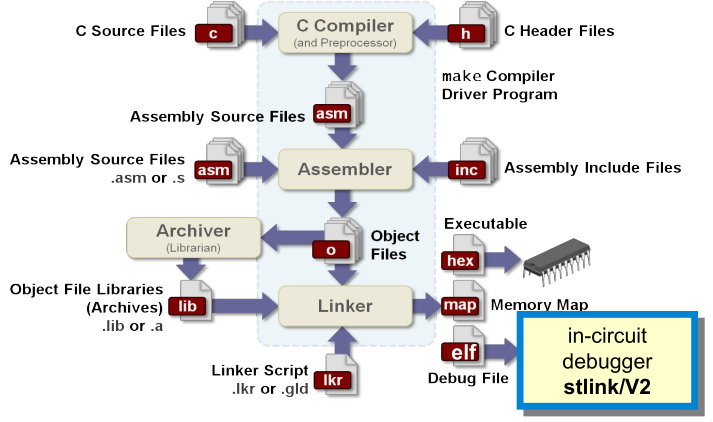
\includegraphics[width=0.8\linewidth]{immagini/programmazione1}
\end{figure}
\begin{enumerate}
    \item \textbf{Preprocessing e Compilazione C} $\rightarrow$ il \textit{preprocessore} espande le macro definite tramite la direttiva \texttt{\#define} e include il contenuto dei file di intestazione specificati con \texttt{\#include}. Il compilatore esegue l'analisi lessicale e sintattica del codice sorgente (\texttt{.c}) e genera i corrispondenti file sorgente in linguaggio assembly (\texttt{.asm}).
    \item \textbf{Assemblaggio} $\rightarrow$ l'\textit{assembler} elabora i file assembly (\texttt{.asm}, \texttt{.s}) e gli eventuali file ausiliari di inclusione (\texttt{.inc}), traducendoli in file oggetto (\texttt{.o}). I file oggetto contengono codice macchina non ancora consolidato, caratterizzato da riferimenti simbolici non risolti. Per ogni file sorgente C corrisponde un singolo file oggetto; in questa fase possono operare più compilatori e assembler in parallelo.
    \item \textbf{Archiviazione delle librerie} $\rightarrow$ tramite il programma archiver (\textit{librarian}), i file oggetto possono essere raggruppati in librerie di archivi statici (\texttt{.a}) o dinamici (\texttt{.lib}).
    \item \textbf{Linking} $\rightarrow$ un unico \textit{linker} riceve la totalità dei file oggetto (\texttt{.o}), le librerie di sistema o utente (\texttt{.lib}, \texttt{.a}) e le direttive del Linker Script (\texttt{.lkr} o \texttt{.gld}). Il linker unifica i moduli, associa gli indirizzi fisici effettivi a tutti i simboli (funzioni e variabili globali/esterne) e colloca le sezioni di memoria secondo la mappa dell'architettura.
\end{enumerate}

I prodotti generati al termine del linking comprendono:
\begin{itemize}
    \item \textbf{File Eseguibile (\texttt{.hex})} $\rightarrow$ immagine binaria destinata alla scrittura fisica all'interno della memoria del microcontrollore.
    \item \textbf{Memory Map (\texttt{.map})} $\rightarrow$ documento descrittivo recante la ripartizione dettagliata e la collocazione degli indirizzi di memoria assegnati alle sezioni e ai simboli.
    \item \textbf{File di Debug (\texttt{.elf})} $\rightarrow$ formato che include il codice eseguibile integrato con la tabella dei simboli e le informazioni di debug, destinato agli strumenti di ispezione.
\end{itemize}

Il debugger (\textit{in-circuit debugging}) si avvale di una combinazione di elementi hardware e software interfacciati al microcontrollore tramite sonde dedicate (come il modulo hardware ST-Link/V2).

L'analisi degli errori generati durante il flusso consente di isolare la fase di generazione responsabile:
\begin{itemize}
    \item \textbf{Syntax error} $\rightarrow$ errore rilevato dal compilatore dovuto a violazioni della sintassi formale nel codice sorgente C.
    \item \textbf{Unresolved symbol} $\rightarrow$ errore segnalato dal linker causato dall'impossibilità di risolvere l'indirizzo di una funzione o di un identificatore (a causa di nomi errati, funzioni non implementate, moduli omessi in compilazione o librerie mancanti).
\end{itemize}

\subsection{Runtime Startup Code e Avvio del Sistema}
Il software caricato all'interno della memoria di un microcontrollore non è formato solo dal codice scritto dall'utente o generato da configuratori grafici (quali STM32CubeMX), ma include il codice di \textbf{runtime C} e il \textbf{runtime startup code}:
\begin{itemize}
	\item \textbf{C Runtime (CRT)} $\rightarrow$ insieme di routine a basso livello e funzioni di supporto necessarie per il corretto funzionamento del linguaggio C su piattaforma embedded; viene collegato automaticamente in fase di linking e si presenta tipicamente sotto forma di sorgente assembly (\texttt{crt0.s}, oppure file nominati \texttt{startup\_....s} in ambiente ST) o codice oggetto precompilato (\texttt{crt0.o}). 
	
	\item \textbf{Runtime Startup Code} $\rightarrow$ viene eseguito dal processore immediatamente all'uscita dal reset, prima dell'ingresso nella funzione \texttt{main()}. Esso è interamente modificabile dallo sviluppatore qualora siano richieste riconfigurazioni dell'ambiente di esecuzione.
\end{itemize}  
\begin{figure}[H]
	\centering
	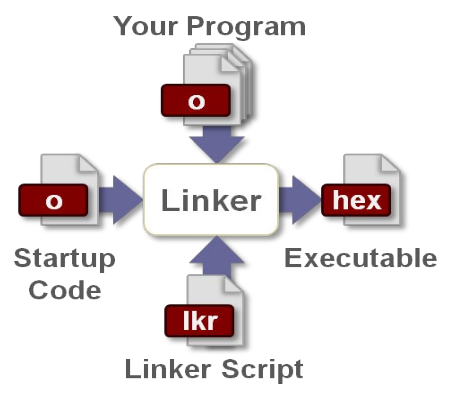
\includegraphics[width=0.35\linewidth]{immagini/programmazione2}
\end{figure}
Le operazioni sequenziali eseguite dal runtime startup code sono:
\begin{enumerate}
    \item Definizione e inizializzazione della tabella dei vettori di interruzione (Interrupt Vector Table, IVT).
    \item Configurazione degli handler per la gestione delle eccezioni hardware e software (condizioni anomale quali divisioni per zero o tentativi di accesso non valido in memoria).
    \item Gestione del vettore di reset: all'indirizzo fisico $0$ della memoria risiede il puntatore all'istruzione di reset, la quale provvede ad azzerare il registro Program Counter (PC), indirizzandolo alla prima istruzione eseguibile.
    \item Inizializzazione fisica di tutte le sezioni di memoria dati (copia dei valori iniziali delle variabili dalla memoria non volatile alla RAM e azzeramento dell'area BSS).
    \item Caricamento e inizializzazione del registro Stack Pointer e delimitazione dello spazio riservato all'Heap.
    \item Salto incondizionato alla prima istruzione della funzione \texttt{main()}.
\end{enumerate}

\newpage
\section{Struttura del programma e sintassi fondamentale}
Un programma in C destinato a sistemi embedded presenta una struttura modulare governata da direttive e blocchi funzionali:
\begin{minted}[linenos]{c}
#include <stdio.h>

#define PI 3.14159

int main(void)
{
	float radius, area;
	//Calculate area of circle
	radius = 12.0;
	area = PI * radius * radius;
	printf("Area = %f", area);
}
\end{minted}
\begin{itemize}
    \item \textbf{\texttt{\#include <stdio.h>}} $\rightarrow$ direttiva per il preprocessore deputata a includere integralmente nel sorgente il contenuto del file header standard, rendendo disponibili i prototipi delle funzioni di I/O.
    \item \textbf{\texttt{\#define PI 3.14159}} $\rightarrow$ direttiva per la sostituzione testuale; ogni occorrenza dell'etichetta nel codice sottostante viene sostituita letteralmente con il valore definito prima della compilazione.
    \item \textbf{\texttt{int main(void)}} $\rightarrow$ funzione principale obbligatoria; ogni applicativo C deve presentare una e una sola funzione \texttt{main()}, punto di avvio del codice utente al completamento del setup del CRT.
\end{itemize}

Nelle applicazioni embedded su architetture ARM, le funzioni di libreria standard per la stampa a video (come \texttt{printf()}) possono operare mediante la modalità di \textbf{semihosting}. Il semihosting è un meccanismo hardware/software che permette al firmware in esecuzione sul microcontrollore di impiegare i canali di input/output della macchina host che ospita il debugger; per realizzare la console/terminale viene impiegata direttamente una delle linee di debug hardware, evitando l'allocazione e l'occupazione di una linea seriale fisica del microcontrollore.

Il linguaggio C supporta due tipologie di \textbf{commenti}:
\begin{itemize}
    \item Commenti a blocco: delimitati all'apertura da \texttt{/*} e in chiusura da \texttt{*/}, possono estendersi su più righe di testo.
    \item Commenti a singola linea: introdotti dalla sequenza \texttt{//}, estendono il commento fino al termine della riga corrente.
\end{itemize}

Gli \textbf{identificatori} definiscono i nomi univoci attribuiti a elementi quali variabili, funzioni o array per referenziarli prescindendo dall'effettiva locazione di memoria. Le regole sintattiche stabiliscono che:
\begin{itemize}
    \item Gli identificatori devono essere costituiti da sequenze di caratteri.
    \item Il primo carattere non deve essere un numero.
    \item È fatto divieto assoluto di includere caratteri di spaziatura.
    \item La sintassi è rigorosamente case sensitive (es. \texttt{myVar} e \texttt{MyVar} identificano due entità differenti).
\end{itemize}

Lo standard ANSI C definisce un insieme di parole chiave riservate (\textit{keywords}) che possiedono un significato sintattico specifico per il compilatore e non possono in alcun caso essere impiegate come identificatori:
\begin{itemize}
	\item \texttt{auto}: dichiara una variabile locale con allocazione e durata automatica (comportamento predefinito nelle funzioni).
	\item \texttt{break}: interrompe l'esecuzione del ciclo (\texttt{for}, \texttt{while}, \texttt{do-while}) o del blocco \texttt{switch} corrente.
	\item \texttt{case}: definisce una specifica etichetta di valore all'interno di un'istruzione \texttt{switch}.
	\item \texttt{char}: tipo di dato fondamentale per rappresentare singoli caratteri o interi su 1 byte.
	\item \texttt{const}: qualifica una variabile come di sola lettura, impedendone la modifica successiva.
	\item \texttt{continue}: salta il resto dell'iterazione corrente di un ciclo e passa alla successiva.
	\item \texttt{default}: definisce il ramo di fallback in uno \texttt{switch} nel caso nessun \texttt{case} corrisponda.
	\item \texttt{do}: avvia un ciclo a controllo post-condizionale in coppia con \texttt{while} (eseguito almeno una volta).
	\item \texttt{double}: tipo di dato per numeri in virgola mobile a doppia precisione (64 bit).
	\item \texttt{else}: definisce il blocco alternativo da eseguire quando la condizione dell'\texttt{if} risulta falsa.
	\item \texttt{enum}: definisce un tipo di dato per enumerazione, associando identificatori a costanti intere.
	\item \texttt{extern}: dichiara una variabile o funzione la cui definizione effettiva si trova in un'altra unità di traduzione.
	\item \texttt{float}: tipo di dato per numeri in virgola mobile a singola precisione (32 bit).
	\item \texttt{for}: struttura di controllo per cicli composti da inizializzazione, condizione di permanenza e passo di incremento.
	\item \texttt{goto}: esegue un salto incondizionato verso un'etichetta (\textit{label}) definita all'interno della stessa funzione.
	\item \texttt{if}: costrutto condizionale che esegue un blocco di istruzioni solo se l'espressione di test è vera.
	\item \texttt{int}: tipo di dato fondamentale per la rappresentazione di numeri interi con segno.
	\item \texttt{long}: modificatore o tipo di dato per rappresentare interi (o float) con intervallo di valori esteso.
	\item \texttt{register}: suggerisce al compilatore di allocare la variabile direttamente in un registro CPU per minimizzare i tempi di accesso.
	\item \texttt{return}: termina l'esecuzione della funzione corrente e restituisce un eventuale valore al chiamante.
	\item \texttt{short}: modificatore o tipo di dato per interi di dimensione e intervallo ridotti rispetto a \texttt{int}.
	\item \texttt{signed}: specifica esplicitamente che un tipo intero memorizza sia valori positivi che negativi.
	\item \texttt{sizeof}: operatore valutato a tempo di compilazione che restituisce la dimensione in byte di un tipo o variabile.
	\item \texttt{static}: mantiene persistente il valore di variabili locali tra chiamate successive, oppure limita lo \textit{scope} di variabili/funzioni globali al singolo modulo.
	\item \texttt{struct}: definisce un tipo di dato eterogeneo composto da più membri memorizzati contiguamente.
	\item \texttt{switch}: costrutto di selezione multipla che devia il flusso in base al valore intero di un'espressione.
	\item \texttt{typedef}: definisce un alias o sinonimo per un tipo di dato preesistente.
	\item \texttt{union}: definisce una struttura dati in cui tutti i membri condividono la medesima area di memoria sovrapposta.
	\item \texttt{unsigned}: specifica che un tipo intero gestisce unicamente valori non negativi ($\ge 0$).
	\item \texttt{void}: indica un tipo nullo o vuoto, usato per funzioni senza valore di ritorno o puntatori generici privi di tipo tipizzato.
	\item \texttt{volatile}: segnala al compilatore che il valore può variare in modo asincrono (es. registri mappati su hardware o routine ISR), inibendo l'ottimizzazione sui registri.
	\item \texttt{while}: costrutto iterativo a controllo pre-condizionale che reitera finché l'espressione si mantiene vera.
\end{itemize}

\subsection{Tipizzazione dei dati e dichiarazione delle variabili}
Una \textbf{variabile} costituisce l'associazione tra un tipo di dato e un identificatore, atta a rappresentare una o più locazioni di memoria destinate a contenere le informazioni del programma. Nel linguaggio C ogni variabile deve essere dichiarata prima del suo utilizzo.

Il tipo di dato assolve a due compiti distinti:
\begin{itemize}
    \item Specifica al linker il quantitativo di memoria da riservare per la memorizzazione della variabile.
    \item Specifica al compilatore le regole di manipolazione e le operazioni lecite sul dato memorizzato.
\end{itemize}

I tipi di dato fondamentali e la loro occupazione di memoria sono:
\begin{itemize}
    \item \textbf{\texttt{char}} $\rightarrow$ carattere singolo, dimensione pari a $8\text{ bit}$.
    \item \textbf{\texttt{int}} $\rightarrow$ valore intero, dimensione pari a $32\text{ bit}$.
    \item \textbf{\texttt{float}} $\rightarrow$ numero in virgola mobile a singola precisione, dimensione pari a $32\text{ bit}$.
    \item \textbf{\texttt{double}} $\rightarrow$ numero in virgola mobile a doppia precisione, dimensione pari a $64\text{ bit}$.
\end{itemize}

I tipi fondamentali possono essere modificati tramite i prefissi \textbf{qualificatori}: \texttt{signed}, \texttt{unsigned}, \texttt{short} e \texttt{long}. Quando il tipo è modificato da un qualificatore, la specificazione del termine \texttt{int} diviene facoltativa (es. \texttt{unsigned} equivale a \texttt{unsigned int}).

La classificazione dei tipi interi qualificati definisce i seguenti intervalli numerici e dimensioni:
\begin{itemize}
    \item \textbf{\texttt{char}}, \textbf{\texttt{signed char}} $\rightarrow$ $8\text{ bit}$, intervallo da $-128$ a $127$.
    \item \textbf{\texttt{unsigned char}} $\rightarrow$ $8\text{ bit}$, intervallo da $0$ a $255$.
    \item \textbf{\texttt{short int}}, \textbf{\texttt{signed short int}} $\rightarrow$ $16\text{ bit}$, intervallo da $-32768$ a $32767$.
    \item \textbf{\texttt{unsigned short int}} $\rightarrow$ $16\text{ bit}$, intervallo da $0$ a $65535$.
    \item \textbf{\texttt{int}}, \textbf{\texttt{signed int}} $\rightarrow$ $32\text{ bit}$, intervallo da $-2^{31}$ a $2^{31}-1$.
    \item \textbf{\texttt{unsigned int}} $\rightarrow$ $32\text{ bit}$, intervallo da $0$ a $2^{32}-1$.
    \item \textbf{\texttt{long int}}, \textbf{\texttt{signed long int}} $\rightarrow$ $32\text{ bit}$, intervallo da $-2^{31}$ a $2^{31}-1$.
    \item \textbf{\texttt{unsigned long int}} $\rightarrow$ $32\text{ bit}$, intervallo da $0$ a $2^{32}-1$.
    \item \textbf{\texttt{long long int}}, \textbf{\texttt{signed long long int}} $\rightarrow$ $64\text{ bit}$, intervallo da $-2^{63}$ a $2^{63}-1$.
    \item \textbf{\texttt{unsigned long long int}} $\rightarrow$ $64\text{ bit}$, intervallo da $0$ a $2^{64}-1$.
\end{itemize}

Per le tipologie in virgola mobile valgono le seguenti estensioni e valori assoluti minimi e massimi:
\begin{itemize}
    \item \textbf{\texttt{float}} $\rightarrow$ $32\text{ bit}$, minimo assoluto $\pm\sim 10^{-44.85}$, massimo assoluto $\pm\sim 10^{38.53}$.
    \item \textbf{\texttt{double}} $\rightarrow$ $64\text{ bit}$, minimo assoluto $\pm\sim 10^{-323.3}$, massimo assoluto $\pm\sim 10^{308.3}$.
    \item \textbf{\texttt{long double}} $\rightarrow$ $64\text{ bit}$, minimo assoluto $\pm\sim 10^{-323.3}$, massimo assoluto $\pm\sim 10^{308.3}$.
\end{itemize}

Sotto il profilo sintattico, si distinguono due \textbf{modalità di dichiarazione}:
\begin{itemize}
    \item \textbf{Dichiarazione} $\rightarrow$ viene associato il tipo all'identificatore senza assegnazione contestuale di valore (es. \texttt{int x, y, z;}, \texttt{float warpFactor;}, \texttt{char text\_buffer[10];}, \texttt{unsigned index;}).
    \item \textbf{Dichiarazione con definizione} $\rightarrow$ contestualmente alla dichiarazione viene assegnato un valore esplicito mediante l'operatore di assegnazione \texttt{=} (es. \texttt{unsigned y = 12;}, \texttt{long int myVar = 0x12345678;}, \texttt{char first = 'a', second, third = 'c';}, in cui solo \texttt{first} e \texttt{third} risultano inizializzate).
\end{itemize}

\section{Organizzazione della memoria e classi di memorizzazione}
Lo spazio di indirizzamento della memoria è organizzato in segmenti funzionali distinti, disposti convenzionalmente dagli indirizzi bassi (\textit{low address}) verso gli indirizzi alti (\textit{high address}):
\begin{figure}[H]
	\centering
	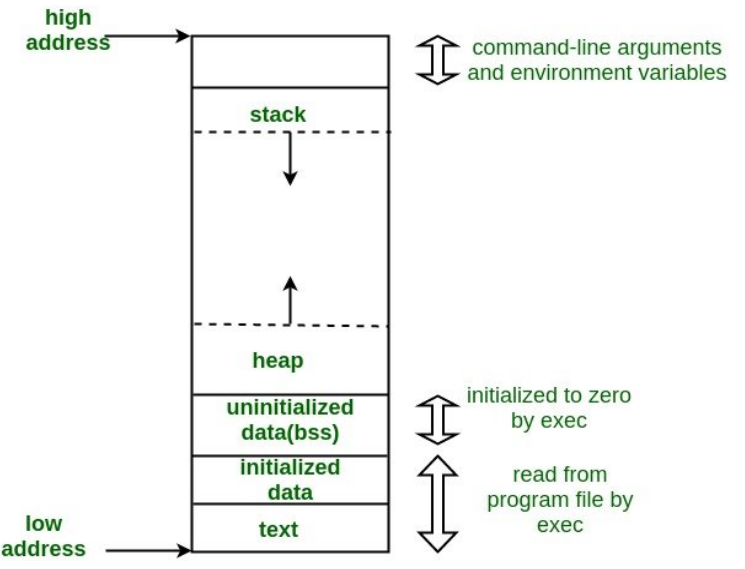
\includegraphics[width=0.5\linewidth]{immagini/programmazione3}
\end{figure}
\begin{itemize}
    \item \textbf{Code Segment (Text Segment)} $\rightarrow$ contiene le istruzioni binarie del programma eseguite dal processore. È un'area ad accesso esclusivo di sola lettura (\textit{read-only}); nei microcontrollori risiede permanentemente nella memoria non volatile (Flash).
    \item \textbf{Data Segment} $\rightarrow$ accoglie le variabili globali e le variabili statiche, suddiviso internamente in due sezioni:
    \begin{itemize}
        \item \textbf{Initialized Data} $\rightarrow$ ospita variabili globali e statiche inizializzate esplicitamente a un valore diverso da zero. Si ripartisce a sua volta in una \textit{read-only area} (costanti e string literal) e una \textit{read-write area}. Nei microcontrollori i valori iniziali risiedono fisicamente in memoria Flash e vengono trasferiti in RAM dallo startup code durante la sequenza di reset, consentendone la modifica a run-time.
        \item \textbf{Uninitialized Data (BSS, Block Started by Symbol)} $\rightarrow$ ospita le variabili globali e statiche non inizializzate o inizializzate esplicitamente a zero; viene azzerato in memoria RAM dal codice di avvio (\texttt{csstartup}) prima dell'avvio dell'applicazione.
    \end{itemize}
    \item \textbf{Heap} $\rightarrow$ destinato all'allocazione dinamica della memoria a run-time mediante le funzioni \texttt{malloc()} e \texttt{free()}; è allocato in RAM e presenta una direzione di crescita verso gli indirizzi alti.
    \item \textbf{Stack} $\rightarrow$ operante in RAM secondo logica LIFO, alloca le variabili locali, le variabili allocate nei registri e l'intero contesto di esecuzione delle funzioni (parametri e indirizzi di ritorno); presenta una direzione di crescita verso il basso (indirizzi decrescenti). Un dimensionamento non idoneo o un eccessivo riempimento dello stack può generare uno sfondamento delle aree contigue fino a raggiungere il Code Segment, costituendo una nota vulnerabilità software.
    \item \textbf{Argomenti da riga di comando e variabili d'ambiente} $\rightarrow$ risiedono al vertice superiore della mappa di memoria, in corrispondenza degli indirizzi più elevati.
\end{itemize}

La dimensione complessiva del programma binario da memorizzare fisicamente è definita dall'espressione:
\[
\text{Codice Binario} = \text{Code Segment} + \text{Initialized Data}
\]

Nei microcontrollori il vettore delle eccezioni è rilocabile; ciò rende possibile rimappare lo spazio di indirizzamento scambiando o modificando le posizioni relative di memoria Flash e RAM.

Le classi di memorizzazione (\textbf{storage classes}) determinano il segmento di allocazione, il valore di inizializzazione predefinito, la visibilità (\textit{scope}) e la persistenza temporale (\textit{life}) delle variabili:

\begin{itemize}
    \item \textbf{\texttt{auto}} $\rightarrow$ allocata nello Stack; assume valore iniziale indefinito (\textit{garbage}); visibilità limitata all'interno del blocco di definizione (\textit{within block}); tempo di vita limitato alla terminazione del blocco (\textit{end of block}).
    \item \textbf{\texttt{extern}} $\rightarrow$ allocata nel Data Segment; valore iniziale predefinito pari a zero; visibilità globale estesa su molteplici file di progetto; tempo di vita esteso all'intera durata dell'esecuzione del programma.
    \item \textbf{\texttt{static}} $\rightarrow$ allocata nel Data Segment; valore iniziale predefinito pari a zero; visibilità confinata al blocco locale in cui è dichiarata (\textit{within block}); tempo di vita permanente per l'intera durata del programma.
    \item \textbf{\texttt{register}} $\rightarrow$ allocata direttamente nei registri interni della CPU; assume valore iniziale indefinito (\textit{garbage}); visibilità limitata al blocco (\textit{within block}); tempo di vita limitato alla fine del blocco.
\end{itemize}
\begin{figure}[H]
	\centering
	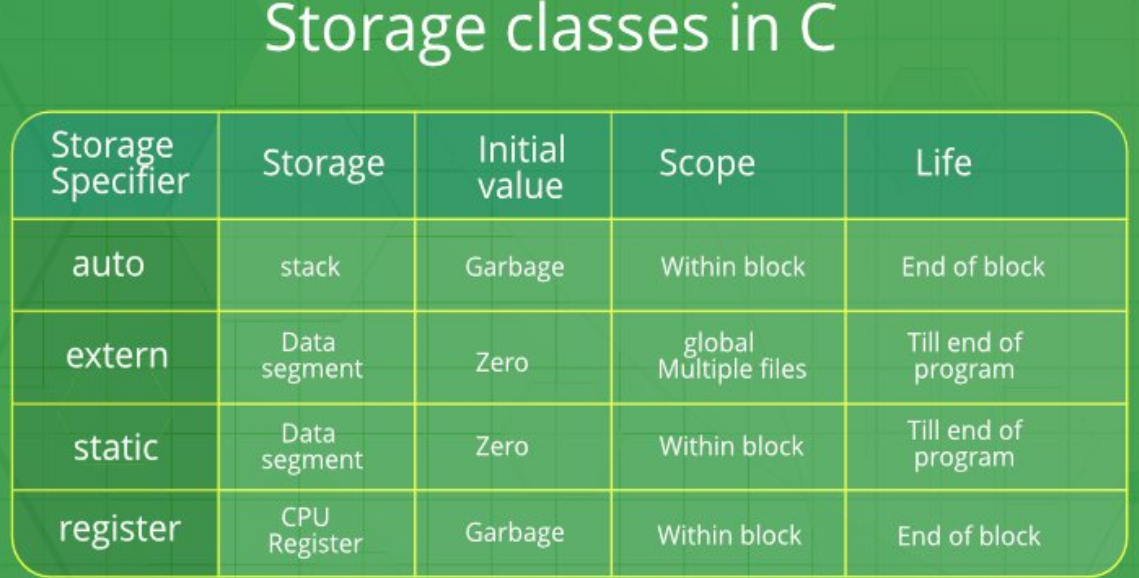
\includegraphics[width=0.7\linewidth]{immagini/programmazione4}
\end{figure}

Le modalità di dichiarazione determinano l'effettivo posizionamento nei segmenti:
\begin{itemize}
    \item Una variabile globale definita con inizializzazione diversa da zero (es. \texttt{int i = 10;}) viene allocata nell'Initialized Data Segment.
    \item Una variabile globale priva di valore iniziale (es. \texttt{int j;}) o qualificata \texttt{static} senza assegnazione (es. \texttt{static int i;}) viene posizionata nel segmento BSS.
    \item L'impiego del modificatore \texttt{static} all'interno di una funzione per una variabile inizializzata (es. \texttt{static int i = 10;}) ne assegna l'allocazione all'Initialized Data Segment, consentendo al dato di preservare il valore tra chiamate successive.
    \item Nella definizione vettoriale \texttt{char s[] = "hello world";}, il dato risiede in Flash e viene interamente copiato in RAM durante il run-time; al contrario, nella dichiarazione puntatore \texttt{const char* string = "hello world";}, la stringa costante letterale è confinata nell'area \textit{read-only} dell'Initialized Data, mentre la variabile puntatore \texttt{string} è allocata nell'area \textit{read-write}.
\end{itemize}
